
%==================================================
\section{ベクトル場と Lie 括弧}
%==================================================
\subsection{ベクトル場と流れ}
\begin{defn}
\emph{ベクトル場}は $TM$ の滑らかな切断 $X:M\to TM$（$\pi\circ X=\id$）。座標で $X=X^i\partial_i$、$X^i$ は滑らかな関数。$X$ は $f\mapsto Xf=X^i\partial_if$ により $C^\infty(M)$ の微分（Leibniz 則を満たす線形作用素）と同一視される。
\end{defn}

$X$ の積分曲線 $\dot\gamma(t)=X(\gamma(t))$ の局所的な族が\emph{流れ} $\varphi_t$（局所1パラメータ群）である。常微分方程式の存在・一意性・滑らかな依存から従う\tC（Lee, 第9章）。例：$\R$ 上の $X=x\partial_x$ の流れは $\varphi_t(x)=e^tx$。$\R^2$ 上の $X=x\partial_y-y\partial_x$ の流れは回転 $\varphi_t(x,y)=(x\cos t-y\sin t,\,x\sin t+y\cos t)$。

\subsection{Lie 括弧}
\begin{defn}[Lie 括弧]
ベクトル場 $X,Y$ に対し $[X,Y]f=X(Yf)-Y(Xf)$。
\end{defn}

\begin{prop}\label{prop:bracket}
\tP\ $[X,Y]$ はまたベクトル場で、座標で $[X,Y]^k=X^i\partial_iY^k-Y^i\partial_iX^k$。さらに
\begin{enumerate}
\item 双線形・反対称：$[X,Y]=-[Y,X]$。
\item Jacobi 恒等式：$[X,[Y,Z]]+[Y,[Z,X]]+[Z,[X,Y]]=0$。
\item Leibniz 則：$[X,fY]=(Xf)Y+f[X,Y]$。
\item 自然性：$F:M\to N$ が微分同相なら $F_*[X,Y]=[F_*X,F_*Y]$。
\end{enumerate}
\end{prop}
\begin{proof}
$X(Yf)-Y(Xf)=X^i\partial_i(Y^j\partial_jf)-Y^i\partial_i(X^j\partial_jf)=(X^i\partial_iY^j-Y^i\partial_iX^j)\partial_jf+X^iY^j\partial_i\partial_jf-Y^iX^j\partial_i\partial_jf$ で、2階の項は $\partial_i\partial_j$ の対称性で打ち消し合う。よって $[X,Y]$ は1階の微分であり、成分は上の式。(1),(3) は定義から直ちに、(2) は6項の展開で全部打ち消し合う（問~\ref{p:jacobi}）。(4) は $F_*X$ が $(F_*X)g=(X(g\circ F))\circ F^{-1}$ で与えられることから従う（問~\ref{p:natural}）。
\end{proof}

つまり $(\X(M),[\,,])$ は無限次元の Lie 代数であり、$C^\infty(M)$ 加群としては Leibniz 則（(3)）を満たす。この「Lie 代数 + Leibniz 則」という構造が、第11巻の \emph{Lie 亜代数}（Lie algebroid）の原型である。

\paragraph{幾何的な意味。}$[X,Y]=\frac{\dd}{\dd t}\big|_{0}(\varphi^X_{-t})_*Y=\Lie_XY$（Lie 微分）\tC\ （Lee, 第9章）。直観的には、$X$ の流れと $Y$ の流れを交互に行っても閉じない量が $[X,Y]$ である。

\begin{figure}[h]
\centering
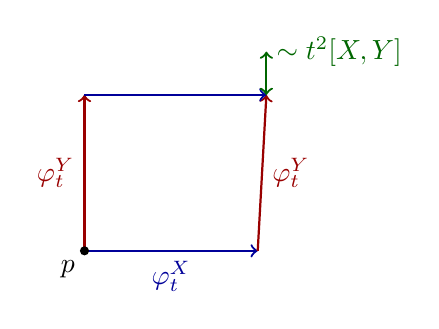
\begin{tikzpicture}[scale=1.1]
\draw[->,thick,blue!60!black] (0,0) -- (2,0) node[midway,below] {$\varphi^X_t$};
\draw[->,thick,red!60!black] (2,0) -- (2.1,1.8) node[midway,right] {$\varphi^Y_t$};
\draw[->,thick,red!60!black] (0,0) -- (0,1.8) node[midway,left] {$\varphi^Y_t$};
\draw[->,thick,blue!60!black] (0,1.8) -- (2.1,1.8+0.0) ;
\draw[<->,thick,green!40!black] (2.1,1.8) -- (2.1,2.3) node[right] {$\sim t^2[X,Y]$};
\fill (0,0) circle (1.5pt) node[below left] {$p$};
\end{tikzpicture}
\caption{流れの交換子：$\varphi^Y_{-t}\varphi^X_{-t}\varphi^Y_t\varphi^X_t(p)$ と $p$ のずれが $t^2[X,Y]$ の程度（厳密な式と符号は規約による。Lee 第9章）。}
\end{figure}


\paragraph{Lie 微分（ベクトル場に対する）。}$X$ の流れ $\varphi_t$ に対し $\Lie_XY=\frac{\dd}{\dd t}\big|_{0}(\varphi_{-t})_*Y$ を $Y$ の $X$ に沿った変化率と定義する。定理 \tC：$\Lie_XY=[X,Y]$。さらに、$[X,Y]=0$ と「$X$ の流れと $Y$ の流れが可換」は同値（Lee 第9章）。したがって座標ベクトル場 $\partial_i$ は互いに可換。逆に、可換で一次独立な $n$ 個のベクトル場は局所座標の座標ベクトル場になる。

\paragraph{Lie 群の場合。}左不変ベクトル場 $X_v$ は左移動（微分同相）で保たれるので、自然性（命題~\ref{prop:bracket}(4)）から $[X_v,X_w]$ も左不変。これにより $T_eG$ に Lie 括弧 $[v,w]:=[X_v,X_w]_e$ が入り、\emph{Lie 代数} $\mathfrak g$ が得られる。例~\ref{ex:so3} の $L_i$ は $SO(3)$ の $\R^3$ への作用の無限小生成元で、$\mathfrak{so}(3)$ の基底の括弧関係を与える（符号は規約による）。

\begin{ex}\label{ex:so3}
$\R^3$ 上の回転のベクトル場 $L_1=y\partial_z-z\partial_y$, $L_2=z\partial_x-x\partial_z$, $L_3=x\partial_y-y\partial_x$ は $[L_1,L_2]=-L_3$, $[L_2,L_3]=-L_1$, $[L_3,L_1]=-L_2$ を満たす（$\mathfrak{so}(3)$。問~\ref{p:so3}）。
\end{ex}

\subsection{分布と Frobenius}
接束の部分束 $D\subset TM$（階数 $k$）が\emph{包合的}とは、$D$ の切断 $X,Y$ に対し $[X,Y]$ も $D$ の切断になること。

\begin{thm}[Frobenius]\tC
階数 $k$ の分布 $D$ が包合的であることと、各点の近傍の座標 $(x^1,\dots,x^n)$ で $D=\mathrm{span}(\partial_1,\dots,\partial_k)$ となること（\emph{可積分}）は同値。
\end{thm}
\src{Lee 第19章、Warner 第1章。証明は流れの可換性を使う。}


\paragraph{Frobenius の定理の証明のあらすじ。}$k=1$ のときは、ベクトル場の流れ箱定理（$X\ne0$ なら $X=\partial_1$ となる座標がある）に他ならない。一般の $k$ では、包合性から基底 $X_1,\dots,X_k$ を取り換えて互いに可換にでき、流れ箱を逐次的に作る（Lee 第19章）。「包合的」の条件が必要なのは、座標ベクトル場 $\partial_1,\dots,\partial_k$ が可換だから $[\partial_i,\partial_j]=0\in D$。逆向きが非自明。

\emph{非自明な例（問~\ref{p:contact}）：} $D=\mathrm{span}(\partial_x+y\partial_z,\,\partial_y)\subset T\R^3$ は包合的でない。$[\partial_x+y\partial_z,\partial_y]=-\partial_z\notin D$。この $D$ は $\ker(\dd z-y\,\dd x)$ で、接触構造の最も簡単な例である。

\begin{keybox}{§2 の要点}
\begin{itemize}
\item $[X,Y]=XY-YX$、成分は $X^i\partial_iY^k-Y^i\partial_iX^k$。Jacobi 恒等式、Leibniz 則、微分同相で保たれる。
\item 幾何的には流れの非可換性。$[X,Y]=\Lie_XY$。包合的 $\Leftrightarrow$ 可積分（Frobenius）。
\item \textbf{【あとで使う】}Lie 括弧は第11巻（Lie 亜代数：Lie 括弧 + anchor）、第12巻（Courant 括弧は $[X,Y]$ を $T\oplus T^*$ に拡張したもの：$[X+\xi,Y+\eta]_{\mathrm{Dorfman}}=[X,Y]+\Lie_X\eta-\iota_Y\dd\xi$。符号と規約は\tQ。第12巻で確認）で再登場する。
\end{itemize}
\end{keybox}

\subsection*{問題（§2）}
\begin{prob}{基本}\label{p:bracketcalc}
$\R^2$ 上で、(a) $[\partial_x,\,x^2\partial_y]$、(b) Euler ベクトル場 $E=x\partial_x+y\partial_y$ と回転 $R=x\partial_y-y\partial_x$ の括弧 $[E,R]$ を計算せよ。
\end{prob}
\begin{prob}{基本}\label{p:so3}
例~\ref{ex:so3} の関係 $[L_1,L_2]=-L_3$ を計算で確かめよ（他の2つは巡回置換で同様）。
\end{prob}
\begin{prob}{標準}\label{p:jacobi}
Jacobi 恒等式 $[X,[Y,Z]]+[Y,[Z,X]]+[Z,[X,Y]]=0$ を、$f\in C^\infty(M)$ に作用させて6項を書き下すことで示せ。
\end{prob}
\begin{prob}{標準}\label{p:natural}
微分同相 $F:M\to N$ に対し $F_*X=\dd F\circ X\circ F^{-1}$ とおくと $(F_*X)g=(X(g\circ F))\circ F^{-1}$ であることを示し、$F_*[X,Y]=[F_*X,F_*Y]$ を導け。応用として、極座標 $(r,\theta)$ で $\partial_r=\frac{x\partial_x+y\partial_y}{r}$, $\partial_\theta=x\partial_y-y\partial_x$（$x=r\cos\theta,\ y=r\sin\theta$）として $[\partial_r,\partial_\theta]=0$ を、座標を使わずに確かめよ。
\end{prob}
\begin{prob}{標準}\label{p:contact}
$X=\partial_x+y\partial_z$, $Y=\partial_y$, $\alpha=\dd z-y\,\dd x$ とする。(a) $\alpha(X)=\alpha(Y)=0$。(b) $[X,Y]$ を求め、$\mathrm{span}(X,Y)$ が包合的でないことを示せ。(c) $\dd\alpha(X,Y)=-\alpha([X,Y])$ を確かめ、$\alpha\wedge\dd\alpha\ne0$ を示せ。
\end{prob}
\begin{prob}{発展}\label{p:witt}
円周 $S^1$ 上のベクトル場 $f\partial_\theta$ について $[f\partial_\theta,g\partial_\theta]=(fg'-f'g)\partial_\theta$ を示せ。$e_n=e^{in\theta}\partial_\theta$（複素係数を許す）が $[e_m,e_n]=i(n-m)e_{m+n}$ を満たすことを確かめ、$E=\partial_\theta$, $C=\cos\theta\,\partial_\theta$, $S=\sin\theta\,\partial_\theta$ が張る3次元部分代数の括弧 $[E,C],[E,S],[C,S]$ を求めよ。
\end{prob}
